%%%%%%%%%%%%%%%%%%%%%%%%%%%%%%%%%%%%%%%%%
% Programming/Coding Assignment
% LaTeX Template
%
% This template has been downloaded from:
% http://www.latextemplates.com
%
% Original author:
% Ted Pavlic (http://www.tedpavlic.com)
%
% Note:
% The \lipsum[#] commands throughout this template generate dummy text
% to fill the template out. These commands should all be removed when 
% writing assignment content.
%
% This template uses a Perl script as an example snippet of code, most other
% languages are also usable. Configure them in the "CODE INCLUSION 
% CONFIGURATION" section.
%
%%%%%%%%%%%%%%%%%%%%%%%%%%%%%%%%%%%%%%%%%

%----------------------------------------------------------------------------------------
%	PACKAGES AND OTHER DOCUMENT CONFIGURATIONS
%----------------------------------------------------------------------------------------

\documentclass{article}

\usepackage{fancyhdr} % Required for custom headers
\usepackage{lastpage} % Required to determine the last page for the footer
\usepackage{extramarks} % Required for headers and footers
\usepackage{minted}
\usepackage[usenames,dvipsnames]{color} % Required for custom colors
\usepackage{graphicx} % Required to insert images
\usepackage{subcaption}
\usepackage{listings} % Required for insertion of code
\usepackage{courier} % Required for the courier font
\usepackage{lipsum} % Used for inserting dummy 'Lorem ipsum' text into the template

% Margins
\topmargin=-0.45in
\evensidemargin=0in
\oddsidemargin=0in
\textwidth=6.5in
\textheight=9.0in
\headsep=0.25in

\linespread{1.1} % Line spacing

% Set up the header and footer
\pagestyle{fancy}
\chead{\hmwkClass\ (\hmwkClassTime): \hmwkTitle} % Top center head
%\rhead{\firstxmark} % Top right header
\lfoot{\lastxmark} % Bottom left footer
\cfoot{} % Bottom center footer
\rfoot{Page\ \thepage\ of\ \protect\pageref{LastPage}} % Bottom right footer
\renewcommand\headrulewidth{0.4pt} % Size of the header rule
\renewcommand\footrulewidth{0.4pt} % Size of the footer rule

\setlength\parindent{0pt} % Removes all indentation from paragraphs

%----------------------------------------------------------------------------------------
%	CODE INCLUSION CONFIGURATION
%----------------------------------------------------------------------------------------

\definecolor{MyDarkGreen}{rgb}{0.0,0.4,0.0} % This is the color used for comments
\lstloadlanguages{Perl} % Load Perl syntax for listings, for a list of other languages supported see: ftp://ftp.tex.ac.uk/tex-archive/macros/latex/contrib/listings/listings.pdf
\lstset{language=Perl, % Use Perl in this example
        frame=single, % Single frame around code
        basicstyle=\small\ttfamily, % Use small true type font
        keywordstyle=[1]\color{Blue}\bf, % Perl functions bold and blue
        keywordstyle=[2]\color{Purple}, % Perl function arguments purple
        keywordstyle=[3]\color{Blue}\underbar, % Custom functions underlined and blue
        identifierstyle=, % Nothing special about identifiers                                         
        commentstyle=\usefont{T1}{pcr}{m}{sl}\color{MyDarkGreen}\small, % Comments small dark green courier font
        stringstyle=\color{Purple}, % Strings are purple
        showstringspaces=false, % Don't put marks in string spaces
        tabsize=5, % 5 spaces per tab
        %
        % Put standard Perl functions not included in the default language here
        morekeywords={rand},
        %
        % Put Perl function parameters here
        morekeywords=[2]{on, off, interp},
        %
        % Put user defined functions here
        morekeywords=[3]{test},
       	%
        morecomment=[l][\color{Blue}]{...}, % Line continuation (...) like blue comment
        numbers=left, % Line numbers on left
        firstnumber=1, % Line numbers start with line 1
        numberstyle=\tiny\color{Blue}, % Line numbers are blue and small
        stepnumber=5 % Line numbers go in steps of 5
}

% Creates a new command to include a perl script, the first parameter is the filename of the script (without .pl), the second parameter is the caption
\newcommand{\perlscript}[2]{
\begin{itemize}
\item[]\lstinputlisting[caption=#2,label=#1]{#1.pl}
\end{itemize}
}

%----------------------------------------------------------------------------------------
%	DOCUMENT STRUCTURE COMMANDS
%	Skip this unless you know what you're doing
%----------------------------------------------------------------------------------------

% Header and footer for when a page split occurs within a problem environment
\newcommand{\enterProblemHeader}[1]{
%\nobreak\extramarks{#1}{#1 continued on next page\ldots}\nobreak
%\nobreak\extramarks{#1 (continued)}{#1 continued on next page\ldots}\nobreak
}

% Header and footer for when a page split occurs between problem environments
\newcommand{\exitProblemHeader}[1]{
%\nobreak\extramarks{#1 (continued)}{#1 continued on next page\ldots}\nobreak
%\nobreak\extramarks{#1}{}\nobreak
}

\setcounter{secnumdepth}{0} % Removes default section numbers
\newcounter{homeworkProblemCounter} % Creates a counter to keep track of the number of problems
\setcounter{homeworkProblemCounter}{0}

\newcommand{\homeworkProblemName}{}
\newenvironment{homeworkProblem}[1][Part \arabic{homeworkProblemCounter}]{ % Makes a new environment called homeworkProblem which takes 1 argument (custom name) but the default is "Problem #"
\stepcounter{homeworkProblemCounter} % Increase counter for number of problems
\renewcommand{\homeworkProblemName}{#1} % Assign \homeworkProblemName the name of the problem
\section{\homeworkProblemName} % Make a section in the document with the custom problem count
\enterProblemHeader{\homeworkProblemName} % Header and footer within the environment
}{
\exitProblemHeader{\homeworkProblemName} % Header and footer after the environment
}

\newcommand{\problemAnswer}[1]{ % Defines the problem answer command with the content as the only argument
\noindent\framebox[\columnwidth][c]{\begin{minipage}{0.98\columnwidth}#1\end{minipage}} % Makes the box around the problem answer and puts the content inside
}

\newcommand{\homeworkSectionName}{}
\newenvironment{homeworkSection}[1]{ % New environment for sections within homework problems, takes 1 argument - the name of the section
\renewcommand{\homeworkSectionName}{#1} % Assign \homeworkSectionName to the name of the section from the environment argument
\subsection{\homeworkSectionName} % Make a subsection with the custom name of the subsection
\enterProblemHeader{\homeworkProblemName\ [\homeworkSectionName]} % Header and footer within the environment
}{
\enterProblemHeader{\homeworkProblemName} % Header and footer after the environment
}

%----------------------------------------------------------------------------------------
%	NAME AND CLASS SECTION
%----------------------------------------------------------------------------------------

\newcommand{\hmwkTitle}{Project\ \#2} % Assignment title
\newcommand{\hmwkDueDate}{Friday,\ March\ 10,\ 2017} % Due date
\newcommand{\hmwkClass}{CSC411} % Course/class
\newcommand{\hmwkClassTime}{L0101} % Class/lecture time
\newcommand{\hmwkAuthorName}{Firstname Lastname} % Your name

%----------------------------------------------------------------------------------------
%	TITLE PAGE
%----------------------------------------------------------------------------------------

\title{
\vspace{2in}
\textmd{\textbf{\hmwkClass:\ \hmwkTitle}}\\
\normalsize\vspace{0.1in}\small{Due\ on\ \hmwkDueDate}\\
\vspace{0.1in}
\vspace{3in}
}

\author{\textbf{Fiona Leung} \textit{999766061}
  \\ \textbf{Timur Borkhodoev} \textit{999376394}}
%\date{} % Insert date here if you want it to appear below your name

%----------------------------------------------------------------------------------------

\begin{document}

\maketitle
\clearpage

%----------------------------------------------------------------------------------------
%	PART 1
%----------------------------------------------------------------------------------------
\begin{homeworkProblem}
\noindent \textit{Dataset description}
  The dataset contained an even number of images per digit, having no more or
  less information the neural networks coud train off of determine one digit
  better apart from another. Each digit had multiple images of it where it was
  drawn with varying writing styles. Some digits were written with more loops
  and imperfections than others, had different thicknesses or were drawn slanted
  at different angles.Some digit images had discontinuous lines in the number
  shapes.

  For example, in the images of the 0's some had a closed loop while others were
  perfect and had a small edge that jutted out near its top.
\begin{enumerate}
  \item variety of angles
  \item different styles of handwriting
  \item gaps between continuous lines
  \item different thickness levels
\end{enumerate}
\begin{center}
  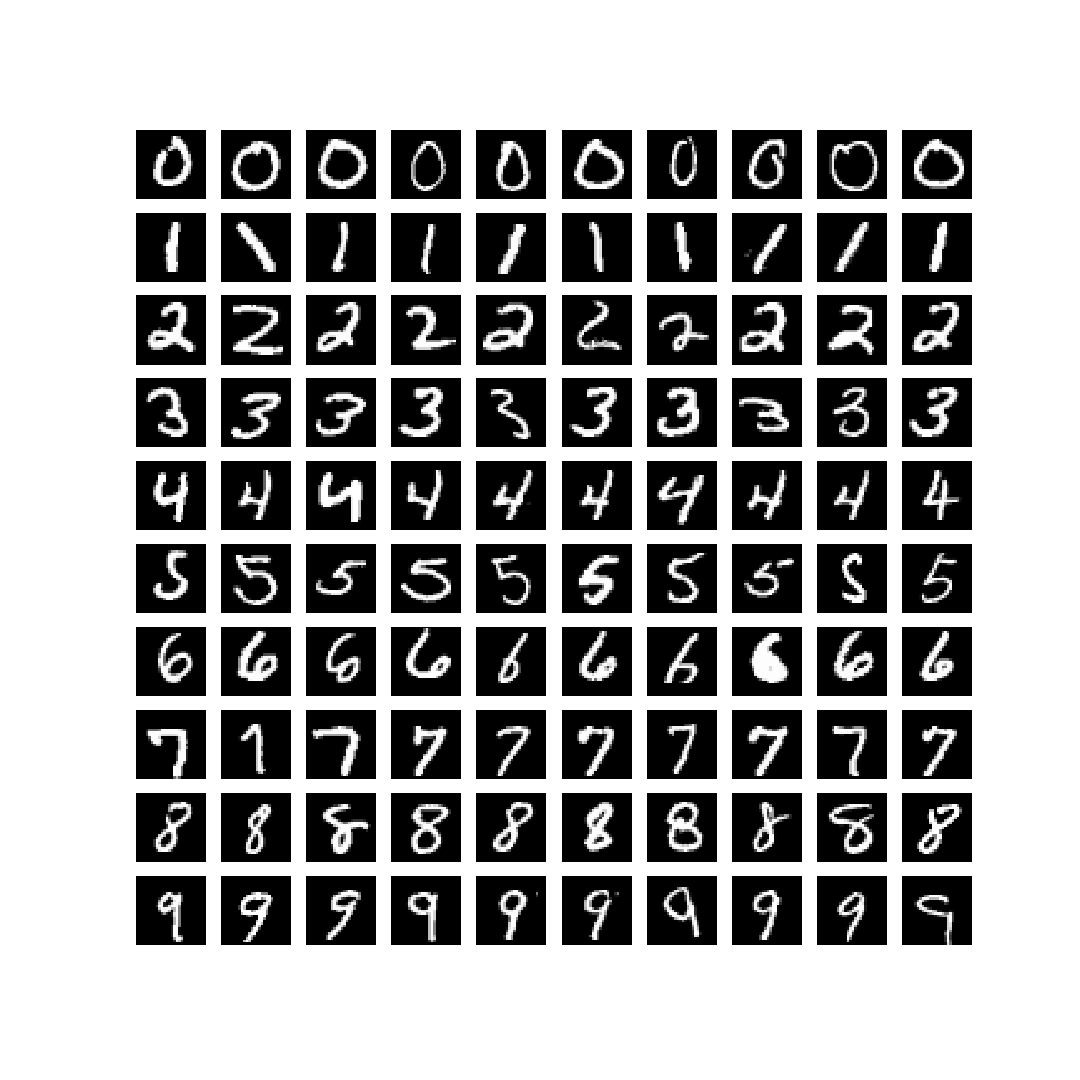
\includegraphics[scale=0.3]{images/dataset.png}
\end{center}
\end{homeworkProblem}
%----------------------------------------------------------------------------------------
%	PART 2
%----------------------------------------------------------------------------------------
\begin{homeworkProblem}
\noindent \textit{Compute the network function by propagating forward and
  discarding intermediate results}
  \begin{minted}[frame=lines, framesep=2mm, baselinestretch=1.2, linenos]{python}
def compute_network(x, W0, b0, W1, b1):
    _,_, output = forward(x, W0, b0, W1, b1)
    return = argmax(output)
\end{minted}
\end{homeworkProblem}
%----------------------------------------------------------------------------------------
%	PART 3 
%----------------------------------------------------------------------------------------
\begin{homeworkProblem}
  \begin{enumerate}
    \item We will use negative log-probabilities as our cost function, and find
      its gradient
  \begin{minted}[frame=lines, framesep=2mm, baselinestretch=1.2, linenos]{python}
def cross_entropy(y, y_):
  return -sum(y_ * log(y))
      \end{minted}
    \item Vectorized code for computing gradient of the cost function
  \begin{minted}[frame=lines, framesep=2mm, baselinestretch=1.2, linenos]{python}
def deriv_multilayer(W0, b0, W1, b1, x, L0, L1, y, y_):
    dCdL1 = y - y_
    dCdW1 = dot(L0, dCdL1.T)
    dCdobydodh = dot(W1, dCdL1)
    diff = 1 - L0**2

    dCdW0 = tile(dCdobydodh, 28 * 28).T * dot(x, (diff.T))
    dCdb1 = dCdL1
    dCdb0 = dCdobydodh * diff

    return dCdW1, dCdb1, dCdW0, dCdb0
      \end{minted}
  \end{enumerate}

To verify gradient correctness we used finite differences to compare our output.
\begin{center}
\begin{tabular}{ |c|c|c| } 
 \hline
 Method& approximation & gradient \\ 
 \hline
 W1 & 0.984191894531 & 0.984342670068 \\ 
 W0 & 0.0 & -0.0 \\ 
 b1 & 0.000476837158203 & 0.000534144113772 \\ 
 b0 & 0.0 & 0.0 \\ 
 \hline
\end{tabular}
\end{center}
\end{homeworkProblem}
%----------------------------------------------------------------------------------------
%	PART 4 
%----------------------------------------------------------------------------------------
\begin{homeworkProblem}
  We start by loading sample weights from the pickle file. Then train it using
  mini-batch optimization to speed up training. Our training method works as follow:
  \begin{enumerate}
  \item First forward method - passes flattened image through the network
    keeping all intermediate results
  \item Then we compute the gradient with respect to $W0,b0,W1,b1$
  \item We keep accumulating error values and then update our parameters
    $W0,b0,W1,b1$ over a single batch and repeat
  \end{enumerate}
  \begin{minted}[frame=lines, framesep=2mm, baselinestretch=1.2, linenos]{python}
def train(plot=False):
    global W0, b0, W1, b1
    global plot_iters, plot_performance
    plot_iters = []
    plot_performance = []
    alpha = 1e-3
    for i in range(150):
        X, Y, examples_n = get_batch(i * 5,10)

        update = np.zeros(4)

        for j in range(examples_n):
            y = Y[j].reshape((10, 1))
            x = X[j].reshape((28 * 28, 1)) / 255.
            L0, L1, output = forward(x, W0, b0, W1, b1)
            gradients = deriv_multilayer(W0, b0, W1, b1, x, L0, L1, output, y)
            update = [update[k] + gradients[k] for k in range(len(gradients))]

        # update the weights 
        W1 -= alpha * update[0]
        b1 -= alpha * update[1]
        W0 -= alpha * update[2]
        b0 -= alpha * update[3]
        if plot:
            plot_iters.append(i * examples_n)
            plot_performance.append(test_perf())
    return plot_iters,plot_performance
train(plot=True)
      \end{minted}
    \begin{minted}[frame=lines, framesep=2mm, baselinestretch=1.2, linenos]{python}
def get_batch(offset,example_per_class=5):
    # 5 examples per class
    classes_num = 10
    x_batch = np.zeros((example_per_class * classes_num, 28 * 28))
    y_batch = np.zeros((example_per_class * classes_num, classes_num))
    for i in range(classes_num):
        for j in range(example_per_class):
            x_batch[i * example_per_class + j] = M['train' + str(i)][j +
                                                                     offset]
            y_batch[i * example_per_class + j][i] = 1
    return x_batch, y_batch, example_per_class * classes_num
\end{minted}
  \pagebreak
  \begin{center}
    visualizing weights:\\
    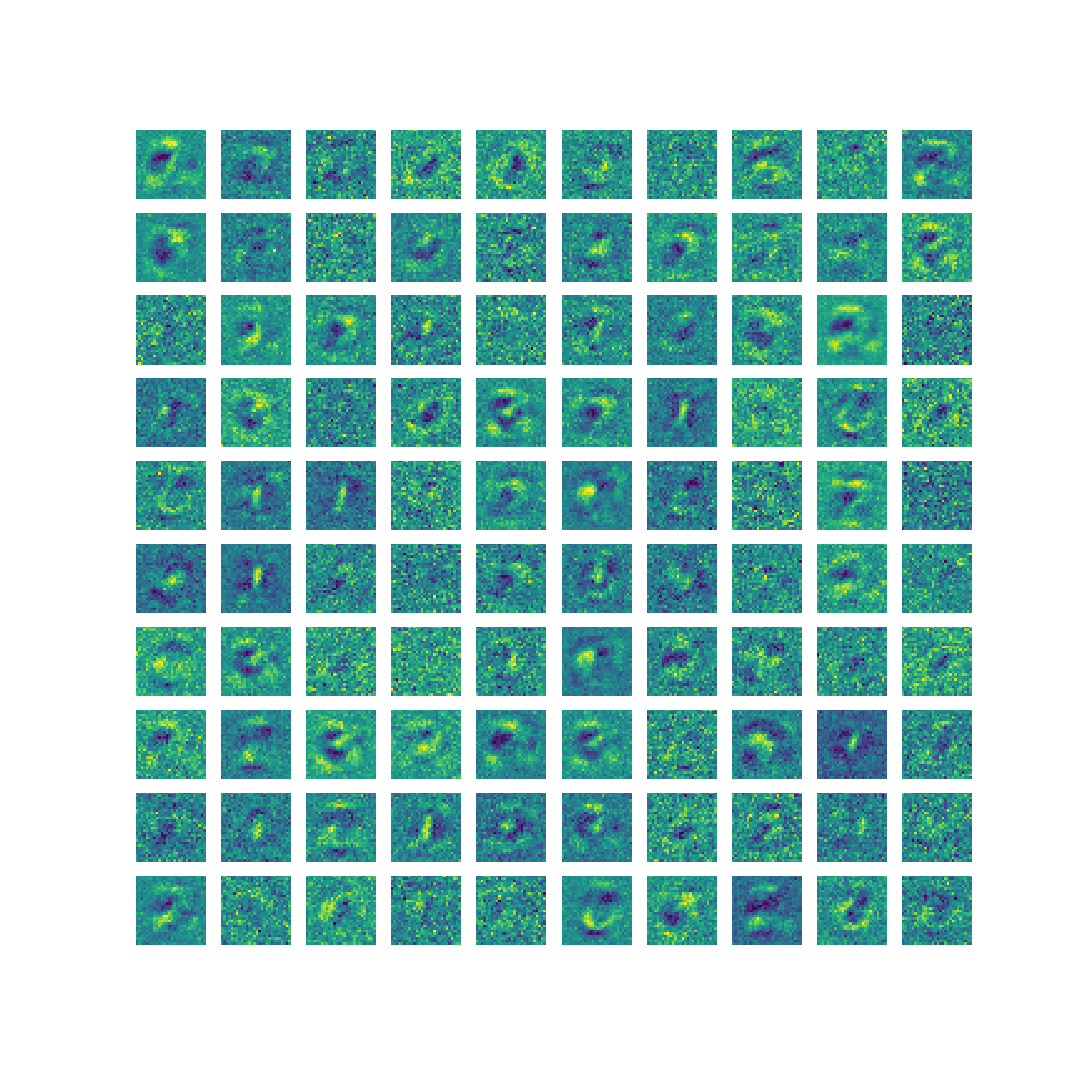
\includegraphics[scale=0.4]{images/weights.png}\\
    performance graph:\\
    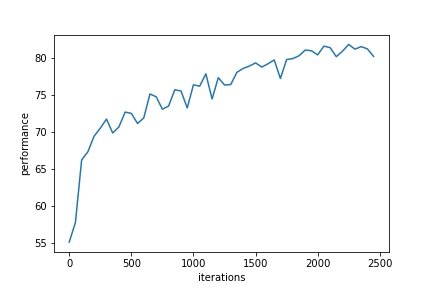
\includegraphics[scale=0.8]{images/performance.png}
  \begin{center}
\end{homeworkProblem}
%----------------------------------------------------------------------------------------
%	PART 5 
%----------------------------------------------------------------------------------------
\begin{homeworkProblem}
  So as discussed in lecture large errors are penalized quadratically in linear
  regressions. So our multinomial regression doesn't suffer from it. We start
  with generating a noise for our data set. 
  \begin{minted}[frame=lines, framesep=2mm, baselinestretch=1.2, linenos, mathescape,gobble=2]{python}
  # generate noise and $N(0, \sigma^2)$
  noise = scipy.stats.norm.rvs(scale=5,size=784*50*10)
  noise = noise.reshape(500,784)
  X,Y,n = get_batch(offset=0,examples=50)
  X += noise
  \end{minted}
  After modifying our data set with noise - we get images that look like this
  \\ 
  
  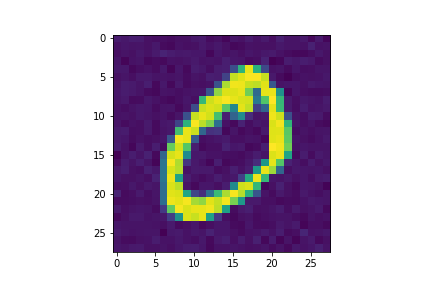
\includegraphics[scale=0.5]{images/noise_image.png}
\end{homeworkProblem}

%----------------------------------------------------------------------------------------
%	PART 7
%----------------------------------------------------------------------------------------
\begin{homeworkProblem}
	
	To construct the neural network, we trained on 5400 images with 90
	images per actor. Each image was cropped to a bounding box that was resized to a $60 \times 60$ array containing only the actor's face. Images were serialized in a dictionary that mapped the actors' names to an array list of their whole RGB images saved in a three-dimensional numpy array.
	
	\begin{verbatim}
		actor_imgs = {
						'Steve Carell': [carell_1, carell_2, ..., carell_n],
						'Fran Drescher': [drescher_1, drescher_2, ..., drescher_n]
					 }
	\end{verbatim}
	
	
	This dictionary was read from a file called \texttt{actor\_imgs.p} using the \texttt{pickle} module to create a unique training, validation and test set.
		
	Each image passed through the neural network was preprocessed to standardize its values and characteristics so we could compare images on the same physical conditions as closely as possible.
	
	
	To preprocess each image we did the following:
	\begin{itemize}
		\item grayscale the image to convert the 3D RGB image to a 2D array \texttt{rgb2gray()} function given in class.
		\item flattening the image array to a $1 \times 786$ vector stored in a NumPy array
		\item normalize the image's pixels, their values are limited to values 0 to 1. This will allow us to compare images by standardizing the range of their pixel intensities
	\end{itemize}
	
	\emph{Neural Network Performance}
	
\end{homeworkProblem}
\end{document}


	
	
\end{document}

